\ylDisplay{Plokid} % Ülesande nimi
{Taavet Kalda} % Autor
{lahtine} % Voor
{2017} % Aasta
{G 8} % Ülesande nr.
{8} % Raskustase
{
% Teema: Dünaamika
\ifStatement
Joonisel on kujutatud kahest plokist ja kolmest raskusest, massidega $m_1$, $m_2$ ja $M$ koosnevat süsteemi. Nöörid on venimatud ning nööride ja plokkide massid on tühised võrreldes raskuste massidega. Hõõre ploki ja nööri vahel on tühiselt väike. Missugune peaks olema $M$ väärtus selleks, et $M$ jääks esialgu paigale, kui süsteem lahti lasta?

\begin{center}
	\vspace{-10pt}
	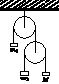
\includegraphics[width = 0.3\linewidth] {2017-lahg-08-double_pulleys_img.pdf}
\end{center}
\fi


\ifHint
Paneme tähele, et niidi pinge alumises nööris on kaks korda väiksem kui ülemises nööris. Selles saab veenduda, kui vaadelda alumisele plokile mõjuvaid jõudusid. Lisaks saab mõlema nööri jaoks kirja panna nende venimatuse tingimuse.
\fi


\ifSolution
Olgu ülemisele ja alumisele plokile toetuvate nööride pinged vastavalt $T_1$ ja $T_2$ ning raskuste $m_1$, $m_2$ ja $M$ kiirendused vastavalt $a_1$, $a_2$ ja $a$ (gravitatsiooniga samasuunalised). Kuna raskus $M$ peab alguses paigal olema, st $a = 0$. Nööride venimatus annab kaks lisatingimust. Esiteks, ülemise nööri venimatusest peab alumise ploki kiirendus olema $-a_1$. Teiseks, alumise nööri venimatusest saab järeldada, et alumine plokk liigub kiirendusega $\frac{a_2 + a}{2} = \frac{a_2}{2} = -a_1$, sest $m_2$ ja $M$ liiguvad keskmiselt sama palju kui alumine plokk. Kuna nöörid on kaalutud, on nende pinge igas punktis sama. Paneme alumise ploki ja iga raskuse jaoks Newtoni 2. seaduse kirja:
\begin{align}
0 &= 2T_2 - T_1,				& &\text{- alumine plokk}\label{Plokid:eq-1}\\
m_1a_1 &= m_1g - T_1,			& &\text{- esimene raskus}\label{Plokid:eq-2}\\
m_2a_2 &= m_2g - T_2,			& &\text{- teine raskus}\label{Plokid:eq-3}\\
0 &= Mg - T_2,					& &\text{- uuritav raskus}\label{Plokid:eq-4}\\
\frac{a_2}{2} &= -a_1.			& &\text{- nööride venimatus\label{Plokid:eq-5}}
\end{align}
Tekkinud võrrandisüsteemis on 5 võrrandit ja 5 tundmatut. Seega on $M$ üheselt määratud.

(\ref{Plokid:eq-1}) ja (\ref{Plokid:eq-4}) annavad $T_2 = Mg$ ja $T_1 = 2Mg$. Asendame (\ref{Plokid:eq-5}) ja saadud seosed võrranditesse (\ref{Plokid:eq-2}) ja (\ref{Plokid:eq-3}):
\begin{align}
m_1a_1 &= m_1g - 2Mg, \label{Plokid:eq-6}\\
-2m_2a_1 &= m_2g - Mg. \label{Plokid:eq-7}
\end{align}
Liidame (\ref{Plokid:eq-6}) ja (\ref{Plokid:eq-7}) kokku kaaludega $\frac{2}{m_1}$ ja $\frac{1}{m_2}$:
\[
0 = 2g - 4\frac{Mg}{m_1} + g - \frac{Mg}{m_2},
\]
ehk
\[
M = \frac{3}{\frac{4}{m_1} + \frac{1}{m_2}} = \frac{3m_1m_2}{4m_2 + m_1}.
\]
\fi


\ifEngStatement
% Problem name: Blocks
In the figure there is depicted a system that consists of two blocks and three weights of masses $m_1$, $m_2$ and $M$. The strings are non-stretchable and the masses of the strings and blocks are insignificant compared to the masses of the weights. The friction between a block and a string is insignificantly small. What has to be the value of $M$ so that $M$ would initially stay still when the system is let free?
\begin{center}
	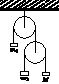
\includegraphics[width = 0.3\linewidth]  {2017-lahg-08-double_pulleys_img.pdf}
\end{center}
\fi


\ifEngHint
Let us notice that the tension of the thread in the bottom string is two times smaller than in the upper one. You can be sure of this if you observe the forces applied to the bottom block. Additionally, you can write down the non-stretchability condition for both of the strings.
\fi


\ifEngSolution
Let the tensions of the strings relying on the upper and bottom block be respectively $T_1$ and $T_2$ and accelerations of the masses $m_1$, $m_2$ and $M$ accordingly $a_1$, $a_2$ and $a$ (with the same direction as the gravity). The mass $M$ has to be still initially, meaning $a = 0$. The non-stretchability of the strings gives two additional conditions. First, from the non-stretchability of the upper string the acceleration of the bottom block has to be $-a_1$. Second, from the non-stretchability of the bottom string we can assume that the bottom block moves with an acceleration $\frac{a_2 + a}{2} = \frac{a_2}{2} = -a_1$ because $m_2$ and $M$ move the same distance on average as the bottom block. Because the strings are weightless they have the same tension on each point. Let us write down the Newton’s second law for the bottom block and each mass:
\begin{align}
0 &= 2T_2 - T_1,				& &\text{- bottom block}\label{Plokid:eq-1}\\
m_1a_1 &= m_1g - T_1,			& &\text{- first mass}\label{Plokid:eq-2}\\
m_2a_2 &= m_2g - T_2,			& &\text{- second mass}\label{Plokid:eq-3}\\
0 &= Mg - T_2,					& &\text{- studied mass}\label{Plokid:eq-4}\\
\frac{a_2}{2} &= -a_1.			& &\text{- non-stretchability of the strings\label{Plokid:eq-5}}
\end{align} 
This system of equations has 5 equations and 5 unknowns. Therefore $M$ is unequivocally determined.\\
(1) and (4) give $T_2 = Mg$ and $T_1 = 2Mg$. We replace (5) and the obtained relations into the equations (2) and (3):
\begin{align}
m_1a_1 &= m_1g - 2Mg, \label{Plokid:eq-6}\\
-2m_2a_1 &= m_2g - Mg. \label{Plokid:eq-7}
\end{align} 
We add (6) and (7) together with the weights $\frac{2}{m_1}$ and $\frac{1}{m_2}$:
\[
0 = 2g - 4\frac{Mg}{m_1} + g - \frac{Mg}{m_2},
\] 
meaning
\[
M = \frac{3}{\frac{4}{m_1} + \frac{1}{m_2}} = \frac{3m_1m_2}{4m_2 + m_1}.
\]
\fi
}